\documentclass[a4paper,norsk, 10pt]{article}
\usepackage[utf8]{inputenc}
\usepackage{verbatim}
\usepackage{listings}
\usepackage{graphicx}
\usepackage[norsk]{babel}
\usepackage{a4wide}
\usepackage{color}
\usepackage{amsmath}
\usepackage{float}
\usepackage{amssymb}
\usepackage[dvips]{epsfig}
\usepackage[toc,page]{appendix}
\usepackage[T1]{fontenc}
\usepackage{cite} % [2,3,4] --> [2--4]
\usepackage{shadow}
\usepackage{hyperref}
\usepackage{titling}
\usepackage{marvosym }
%\usepackage{subcaption}
\usepackage{subfig}
\usepackage[noabbrev]{cleveref}
\usepackage{cite}
\usepackage{todonotes}


\setlength{\droptitle}{-10em}   % This is your set screw

\setcounter{tocdepth}{2}

\lstset{language=c++}
\lstset{alsolanguage=[90]Fortran}
\lstset{alsolanguage=Python}
\lstset{basicstyle=\small}
\lstset{backgroundcolor=\color{white}}
\lstset{frame=single}
\lstset{stringstyle=\ttfamily}
\lstset{keywordstyle=\color{red}\bfseries}
\lstset{commentstyle=\itshape\color{blue}}
\lstset{showspaces=false}
\lstset{showstringspaces=false}
\lstset{showtabs=false}
\lstset{breaklines}
\title{AST5220, Milestone 1}
\author{Daniel Heinesen, daniehei}
\begin{document}
\maketitle

\section{Introduction}
During the next four milestones we are going to calculate the temperature fluctuation of the photons of the \textit{Comic Microwave Background} \footnote{Or to be more precise, the power spectrum of the CMB}. There are many hurdles to overcome on this journey, but the first is the expansion of the space-time in which the photons exist.

The photons we are looking at lives in the same Universe as we do, and from theoretical predictions and observations we know that this Universe is expanding, and has been doing so from the start time, thought the decoupling for matter and photons and all the way to today. As the space and time the photons occupy is expanding the photons will redshift, leading to a decrease in temperature. 
We need a way of quantifying this expansion, to be ables to calculate this change in temperature. We are going to do this by solving the \textit{Friedmann equation}\eqref{eq:Friedmann} to get the Hubble parameter
\begin{equation}\label{eq:H}
H = \frac{\dot{a}}{a},
\end{equation}
where $a$ is the scale factor and $\dot{a}$ its time derivative. The Hubble parameters is an observable quantity which describes the expansion of the Universe. From this we are going to calculate the \textit{conformal time} $\eta$, which is a convenient way of representing cosmic time in many of the equations we are going to solve in later milestones.


\section{Theory}


The main parameters we are looking for is the Hubble parameter \eqref{eq:H} $H$ and the conformal time $\eta$. From Einsteins field equation we can obtain equations for finding $H$, namely the Friedmann equations. We only need the first of these, rewritten as

\begin{equation}\label{eq:Friedmann}
H = H_0 \sqrt{(\Omega_{b,0} + \Omega_{m,0})a^{-3} + (\Omega_{r,0} + \Omega_{\nu,0})a^{-4} + \Omega_{\Lambda,0}},
\end{equation}

where $\Omega_{b,0}, \Omega_{m,0}, \Omega_{r,0}, \Omega_{\nu,0}, \Omega_{\Lambda,0}$ are the \textit{density parameters} for respectively baryons, (cold) dark matter, neutrinos and dark energy. These parameters are given as
\begin{equation}\label{eq:Omega}
\Omega_{x,0} = \frac{\rho_{x,0}}{\rho_{crit,0}} = \rho_{crit,0}\cdot\left[\frac{3H_0^2}{8\pi G}\right]^{-1},
\end{equation}

where $\rho_{x,0}$ is the density and $\rho_{crit,0} = \frac{3H_0^2}{8\pi G}$ is the critical density. Notice that the subscript $0$ means that these are the parameters at present time. If we instead calculate the density and the critical density at a given time, we obtain the density parameter at this time as well. We are going to assume that there are no neutrinos, and set $\Omega_{nu} = 0$ for all times.

To find the $\Omega_{x}$ throughout time, we need the densities. These are gives as
\begin{equation}\label{eq:rho}
\rho_{m} = \rho_{m,0} a^{-3}, \quad \rho_{b} = \rho_{b,0} a^{-3}, \quad \rho_{4} = \rho_{4,0} a^{-4}, \quad \rho_{\Lambda} = \rho_{\Lambda,0}.
\end{equation}

Before going on to look at the conformal time, we are going to define some variables to make our life easier. First, we are not going to have \eqref{eq:Friedmann} as a function of time or the scale factor, but rather over the logarithmic scale factor $x \equiv \ln a = - \ln(1+z)$, where $z$ is the red shift. We are also going to introduce the scaled Hubble parameter $\mathcal{H} \equiv aH$.

We can now find the conformal time $\eta$. From the FRW-line element it is easy to show that one can introduce a new time variable, defines as
\begin{equation}
\frac{d\eta}{dt} = \frac{c}{a}.
\end{equation}
It can be shown that we can rewrite this in another variable
\begin{equation}
\frac{d \eta}{da} = \frac{c}{a\mathcal{H}}.
\end{equation}
Since we have introduces the time parameter $x$, we can rewrite this again
\begin{equation}\label{eq:deta/dx}
\frac{d\eta}{da} = \frac{d\eta}{dx}\frac{dx}{da} = \frac{d\eta}{dx}\frac{d \ln a}{da} = \frac{d\eta}{dx}\frac{1}{a} \Rightarrow \frac{d\eta}{dx} = \frac{c}{a\mathcal{H}}\cdot a = \frac{c}{\mathcal{H}}.
\end{equation}
This makes it easy to integrate to find 

\begin{equation}\label{eq:eta}
\eta(x) = \int_{\log a_{rec}}^{x} \frac{c}{\mathcal{H}} dx.
\end{equation}

We also want to find an expression for $d\mathcal{H}/dx$. This is simply done with our definition of $\mathcal{H}$ and $H$

\begin{equation*}
\frac{d\mathcal{H}}{dx} = \frac{d}{dx}e^x H = e^x \left( H + \frac{dH}{dx}\right) = e^x \left( H + \frac{d}{dx}\left[H_0 \sqrt{(\Omega_{b,0} + \Omega_{m,0})\exp(-3x) + (\Omega_{r,0} + \Omega_{\nu,0})\exp(-4x) + \Omega_{\Lambda,0}}   \right]\right) 
\end{equation*}
\begin{equation}
= e^x\left(H + \frac{H_0^2}{H}\left[-3(\Omega_{b,0} + \Omega_{m,0})\exp(-3x) -4 (\Omega_{r,0} + \Omega_{\nu,0})\exp(-4x)\right] \right)
\end{equation}

\section{Method}

We are going to calculate \eqref{eq:Friedmann} by saying that we are going to look at the universe from the start of the recombination, $z = 1630.4$, to the end of recombination, $z = 614.2$, and from this to today, $z = 0$. We are then going to convert these red shifts into the logarithmic scale factor, and make a grid with $200$ points during recombination and $300$ points after. With this grid we can calculate $H$ from \eqref{eq:Friedmann}.

To find the the conformal time $\eta$ we need a new grid. This time we start with a grid from $a=10^{-10}$ to $a=1$ (today), with 1000 points. To be able to integrate \eqref{eq:deta/dx} we need initial condition for $\eta$ at the start of recombination. We can do this be noting that since we are in a radiation dominated Universe at the start, we can write $a\mathcal{H}(a) \rightarrow H_0\sqrt{\Omega_r}$ as $a\rightarrow 0$. This means that we can make the integral from the start of time, to the initial $a$

\begin{equation}
\eta(a=a_{init}) = \int_0^{a_{init}} \frac{c}{a\mathcal{H}}da \approx \int_0^{a_{init}} \frac{c}{H_0\sqrt{\Omega_r}}da = \frac{c\cdot a_{init}}{H_0\sqrt{\Omega_r}}.
\end{equation}

Thus we have an initial value for $\eta$. To integrate until today we are going to use a ODE solver from Numerical Recipes. We will use a Runge Kutta (qs) \footnote{Can't remember what qs stands for, and can't find a pdf version on the book at the moment...} integrator. 

We want to know $\eta$ at all possible time, not just the ones used here. Thus we use a \textit{spline} on the calculated dataset to find a continuous approximation to $\eta$.



\newpage

\section{Results}


\begin{figure}[ht]
     \centering
     \subfloat[][This shows the Hubble Parameter as a function of the logarithmic scale factor $x$.]{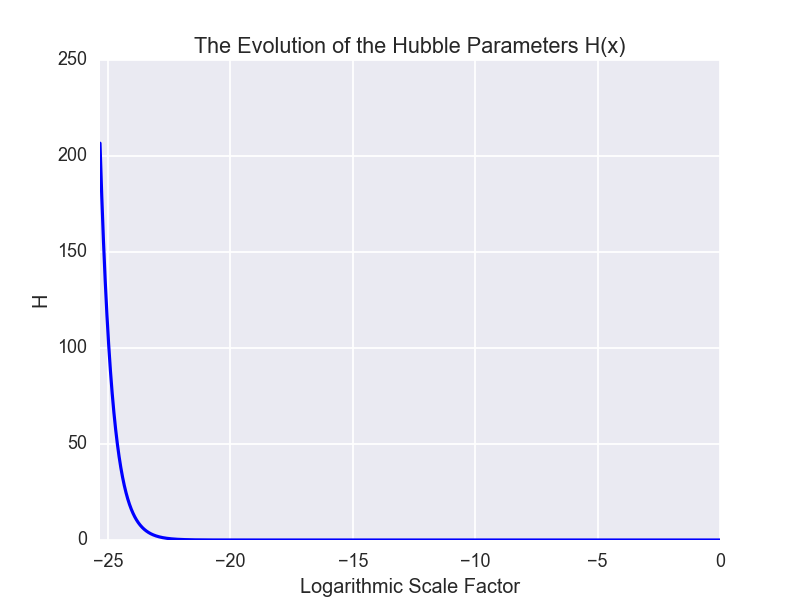
\includegraphics[scale=0.4]{H.png}\label{fig:H}}
     \subfloat[][This shows the Hubble Parameter as a function red shift $z$]{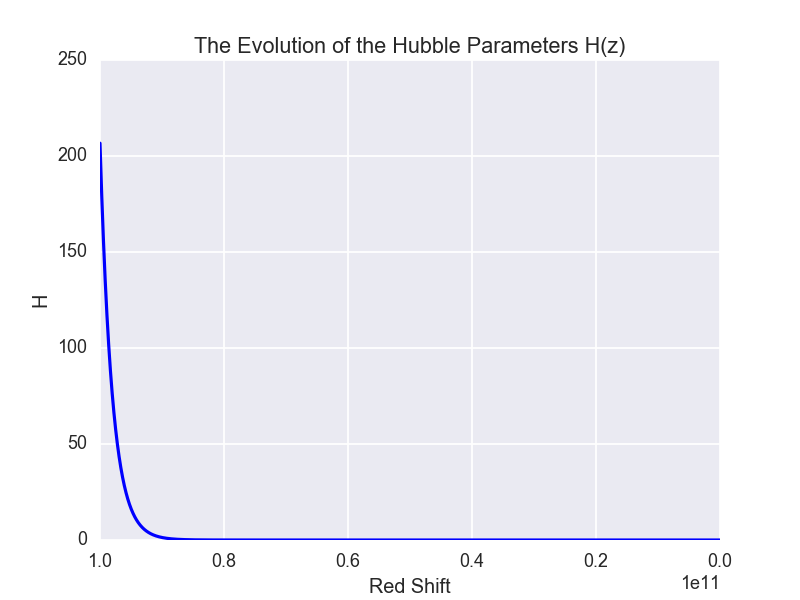
\includegraphics[scale=0.4]{H_z.png}\label{fig:H_z}}
     \caption{These plots show the evolution of the Hubble parameter through the lifetime of the Universe. Notice that for \ref{fig:H} both axes are logged with the natural logarithm. Since \ref{fig:H_z} isn't plotted with a logarithmic variable, no logging of the y-axis is required. This unfortunately makes a direct comparison between the plots less trivial.}
     \label{fig:Hs}
  
\end{figure}



In fig. \ref{fig:Hs} we see the Hubble parameter as a function of the scale factor and red shift. From fig. \ref{fig:H} we see three different epochs, with different slopes. If we look at fig. \ref{fig:omega} we see that these different epochs corresponds domination of the different constituents. If we look at radiation- and matter dominated epochs we know that the Hubble parameters should be $H_{rad} \propto a^{-2}$ and $H_{matter} \propto a^{-3/2}$. This is the same as we see in first two epochs in fig. \ref{fig:H} -- approximately $x < -10$ and $-7<x<-2$--. This indicates that our Hubble parameter is correctly calculated.


\begin{figure}[ht]
     \centering
	{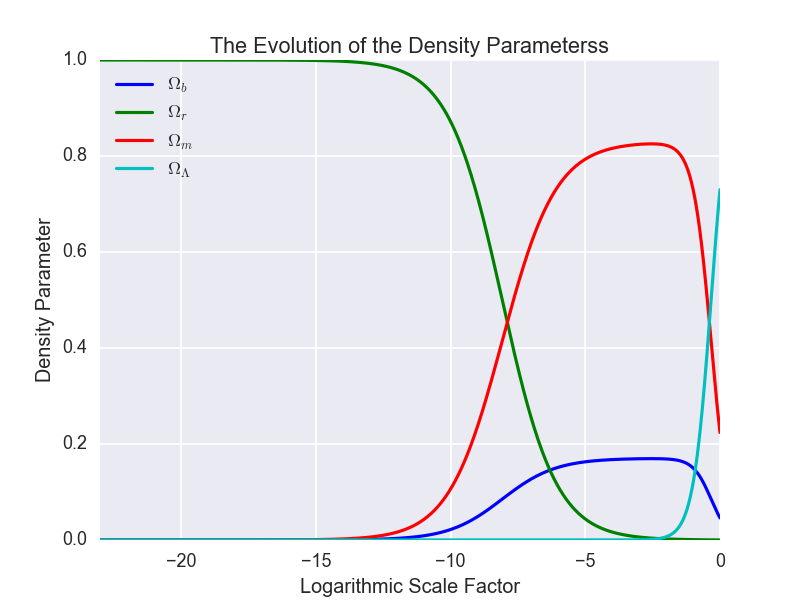
\includegraphics[scale=0.5]{Omega.png}
	\caption{Here we see the evolution of the four density fractions of the Universe. $\Omega_r$ is the density fraction for \textit{radiation}, $\Omega_b$ for \textit{baryons}, $\Omega_b$ for \textit{dark matter}, and $\Omega_{\Lambda}$ for \textit{dark energy}.}\label{fig:omega}}
\end{figure}



Fig. \ref{fig:omega} shows the evolution of the density fraction. From \ref{eq:rho} we see that the different densities have different dependencies on the scale factor $a$. These dependencies also extends to the density fractions \ref{eq:Omega}. Since radiation is dependent on $a^{-4}$, we expect that to be dominant in the early Universe with $a << 1$. This is what we see from fig. \ref{fig:omega}. At some point matter (baryons and dark matter) will be more dominant than radiation due to the fact that $\Omega_{r,0} \approx 10^{-6}$, so even though its dependence on $a^{-4}$ makes it larger that matter( which has a dependence on $a^{-3}$) if $a<1$, this only holds as long as $a < 10^{-6}$, so around this point matter starts to dominate (dark matter in this case, since $\Omega_{b,0}$ is only $0.046$). This is also what we see from the plot. At present time, when $a=1$, we expect that $\Omega_{x,0}$ is the determiner of the values of the densities, which we can see is correct from the figure.


\begin{figure}[H]
     \centering
	{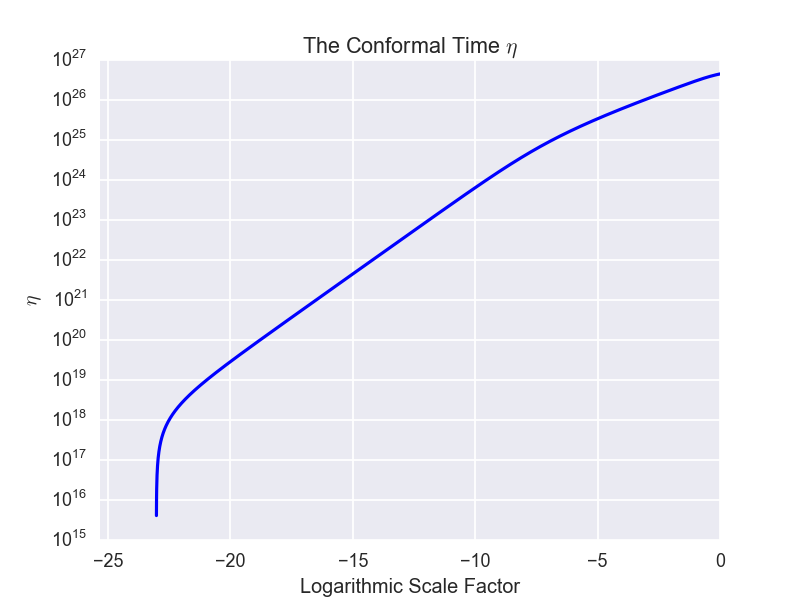
\includegraphics[scale=0.5]{eta.png}
	\caption{Here we can see the conformal time $\eta$ through the lifetime of the Universe. Both the axis are logged with the natural logarithm. The slope of this plot is determined by the type of energy that dominates the Universe. This will be described more in the text. }\label{fig:eta}}
\end{figure}

Fig. \ref{fig:eta} shows the main result of this exercise, the conformal time $\eta$. Once again we see that the plot is divided into the same epochs as seen in fig. \ref{fig:Hs} and fig. \ref{fig:omega}. If we look at the just the radiation- and matter dominated epochs we can find that $\eta_{rad} \propto a$ and $\eta_{matter}\propto \sqrt{a}$. This corresponds well with the slops we see in fig. \ref{fig:eta}.


\section{Conclusion}

Our main result, shown in fig. \ref{fig:eta}, gave us a way of finding a value for the conformal time $\eta$ for a given logarithmic scale factor $x = \log(a)$. We used calculations of the density parameters, fig. \ref{fig:omega}, and estimations of $\eta$ for the different epochs to see that our model was consistent and looked like what we expect from out Universe. 

We also made functions to be able to get values for the Hubble parameter, fig. \ref{fig:Hs}, and for $\mathcal{H}$ and $\frac{d\mathcal{H}}{dx}$, which are not shown in this article.


\end{document}


